% =================================================================================
% DOCUMENT CLASS & PACKAGES
% =================================================================================
\documentclass[11pt, a4paper]{article}

% --- Encoding and Font Packages ---
\usepackage[utf8]{inputenc} % Allows the use of UTF-8 characters

% --- Page Layout Packages ---
\usepackage{geometry}      % For setting page margins
\geometry{a4paper, margin=1in}

% --- Table and List Packages ---
\usepackage{array}         % Provides more advanced column formatting for tables
\usepackage{longtable}     % For tables that span multiple pages

% --- Graphics and Figures ---
\usepackage{graphicx}      % To include images

% --- Header and Footer Packages ---
\usepackage{fancyhdr}      % For custom headers and footers

% =================================================================================
% HEADER & FOOTER CONFIGURATION
% =================================================================================
\pagestyle{fancy}
\fancyhf{} % Clear all header and footer fields
\lhead{Software Requirements Specification for Campus Lost \& Found Portal}
\rfoot{Page \thepage}
\renewcommand{\headrulewidth}{0.4pt} % Adds a rule under the header
\renewcommand{\footrulewidth}{0pt}  % Removes the rule above the footer

% =================================================================================
% TITLE & AUTHOR INFORMATION
% =================================================================================
\title{
    \vspace{2cm} % Add some vertical space at the top
    \textbf{\huge Software Requirements Specification} \\
    \vspace{0.5cm}
    \large for \\
    \vspace{0.5cm}
    \textbf{\Huge Campus Lost \& Found Portal}
    \vspace{2cm}
}

\author{
    Prepared by: \\
    \textbf{Amit Singh \& Priya Sharma} \\
    \textit{School of Computing \& IT} \\
    \textit{Manipal University Jaipur}
}

\date{\textbf{August 3, 2025}}

% =================================================================================
% BEGIN DOCUMENT
% =================================================================================
\begin{document}

% --- Title Page ---
\begin{titlepage}
    \maketitle
    \vfill
    \begin{center}
        \textbf{Version 1.0 approved}
    \end{center}
\end{titlepage}

% --- Table of Contents ---
\pagenumbering{roman} % Start roman numbering for front matter
\tableofcontents
\newpage

% --- Revision History ---
\section*{Revision History}
\begin{tabular}{|m{4cm}|m{3cm}|m{6cm}|m{2cm}|}
    \hline
    \textbf{Name} & \textbf{Date} & \textbf{Reason For Changes} & \textbf{Version} \\
    \hline
    Student 1, Student 2 & 03/08/2025 & Initial Draft & 1.0 \\
    \hline
\end{tabular}
\newpage

% =================================================================================
% MAIN CONTENT - Start Arabic Numbering
% =================================================================================
\pagenumbering{arabic}

% =================================================================================
% SECTION 1: INTRODUCTION
% =================================================================================
\section{Introduction}

\subsection{Purpose}
This Software Requirements Specification (SRS) document outlines the functional and non-functional requirements for the \textbf{Campus Lost \& Found Portal}, version 1.0. This product is a web-based application designed to serve the students and staff of Manipal University Jaipur. Its purpose is to provide a centralized, efficient, and reliable platform for reporting lost items and listing found items within the university campus, thereby simplifying the process of recovering personal belongings.

\subsection{Document Conventions}
This document follows the IEEE 830-1998 standard for SRS documentation. All functional requirements are uniquely identified with a tag of the format \texttt{REQ-X} for traceability. The term "The system" refers to the Campus Lost \& Found Portal software.

\subsection{Intended Audience and Reading Suggestions}
This document is intended for the following audiences:
\begin{itemize}
    \item \textbf{Developers (Project Team):} To understand what needs to be built.
    \item \textbf{Project Manager (Course Instructor):} To oversee the project's progress and ensure it aligns with the course objectives.
    \item \textbf{Testers:} To create test cases based on the specified requirements.
    \item \textbf{University Administration (Stakeholders):} To review the proposed functionality.
\end{itemize}
It is recommended to read the document sequentially, starting with the Introduction and Overall Description to get a high-level overview, followed by the specific System Features and Nonfunctional Requirements for detailed understanding.

\subsection{Product Scope}
The Campus Lost \& Found Portal aims to replace the current informal and fragmented methods of reporting lost items (e.g., physical notice boards, social media groups) with a dedicated digital platform. The key goals are:
\begin{itemize}
    \item To create a single source of truth for all lost and found items on campus.
    \item To reduce the time and effort required for students and staff to find their lost belongings.
    \item To provide an organized and searchable database of items.
    \item To facilitate communication between the person who lost an item and the person who found it.
\end{itemize}
This project is being developed as the minor project for the CS-3230 Software Engineering Lab.

\subsection{References}
\begin{enumerate}
    \item \textit{CS-3230 Software Engineering Lab Course Handout, JAN-MAY 2022, Manipal University Jaipur}.
    \item \textit{Wiegers, Karl E. Software Requirements Specification Template, 1999}.
    \item \textit{Google Material Design Guidelines} (for UI/UX inspiration).
\end{enumerate}

% =================================================================================
% SECTION 2: OVERALL DESCRIPTION
% =================================================================================
\section{Overall Description}

\subsection{Product Perspective}
The Campus Lost \& Found Portal is a new, self-contained product. It will operate as a standalone web application accessible to all members of the university community. It is designed to serve as a central hub, connecting individuals who have lost items with those who have found them, with an administrative layer for oversight.

\subsection{Product Functions}
The major functions of the system are:
\begin{itemize}
    \item User registration and authentication.
    \item Creation and management of "lost item" reports.
    \item Creation and management of "found item" listings.
    \item A comprehensive search and filter functionality for browsing items.
    \item An automated notification system for potential matches.
    \item An administrative dashboard for managing listings and users.
\end{itemize}

\subsection{User Classes and Characteristics}
\begin{longtable}{|p{4cm}|p{11cm}|}
    \hline
    \textbf{User Class} & \textbf{Characteristics} \\
    \hline
    \endfirsthead
    \hline
    \textbf{User Class} & \textbf{Characteristics} \\
    \hline
    \endhead
    \textbf{General User (Student/Staff)} & The primary user class. They can register, log in, report lost items, list found items, search the database, and manage their own posts. They are expected to have basic web literacy and access to a modern web browser. \\
    \hline
    \textbf{Administrator (Campus Admin)} & A privileged user (e.g., from the university's security or administrative department). They can view all listings, remove inappropriate or resolved posts, manage user accounts, and oversee the system's health. \\
    \hline
\end{longtable}

\subsection{Operating Environment}
\begin{itemize}
    \item \textbf{Client-Side:} The system shall be accessible on modern web browsers (Google Chrome, Mozilla Firefox, Safari, Microsoft Edge) on desktop and mobile devices.
    \item \textbf{Server-Side:} The application will be developed using the MERN stack (MongoDB, Express.js, React, Node.js) and deployed on a cloud platform (e.g., Heroku or Vercel).
\end{itemize}

\subsection{Design and Implementation Constraints}
\begin{itemize}
    \item The project must be developed using open-source technologies to avoid licensing costs.
    \item The system must be developed following the Agile/Scrum framework as outlined in the course plan.
    \item All development must be version-controlled using Git and hosted on a shared GitHub repository.
    \item The user interface must be responsive and accessible on both desktop and mobile devices.
    \item The project must be completed within the 12-week semester timeline.
\end{itemize}

\subsection{User Documentation}
The following user documentation will be provided:
\begin{itemize}
    \item An online FAQ page addressing common user questions.
    \item A \texttt{README.md} file in the GitHub repository detailing the project setup and deployment instructions.
\end{itemize}

\subsection{Assumptions and Dependencies}
\begin{itemize}
    \item It is assumed that users will provide accurate information when reporting items.
    \item The system depends on a third-party email service (e.g., SendGrid API) for sending notifications.
    \item It is assumed that the university will provide a designated administrator to manage the system.
\end{itemize}

% =================================================================================
% SECTION 3: EXTERNAL INTERFACE REQUIREMENTS
% =================================================================================
\section{External Interface Requirements}

\subsection{User Interfaces}
The system will feature a clean, modern, and intuitive graphical user interface (GUI). Key screens will include:
\begin{itemize}
    \item \textbf{Homepage:} Displaying recent listings and search functionality.
    \item \textbf{Login/Registration Pages:} For user authentication.
    \item \textbf{Item Submission Form:} A user-friendly form for item details and image upload.
    \item \textbf{Search Results Page:} A filterable and sortable view of all listings.
    \item \textbf{Item Detail Page:} Showing all information for a single item.
    \item \textbf{User Dashboard:} Allowing users to view and manage their own posts.
\end{itemize}

\subsection{Hardware Interfaces}
No direct hardware interfaces are required for this web-based application.

\subsection{Software Interfaces}
The system will interface with an external email gateway API (e.g., SendGrid) to send automated email notifications for registration, password resets, and potential item matches.

\subsection{Communications Interfaces}
All communication between the client (browser) and the server will use the standard HTTPS protocol to ensure data security.

% =================================================================================
% SECTION 4: SYSTEM FEATURES
% =================================================================================
\section{System Features}

% --- Feature 1: User Account Management ---
\subsection{System Feature 1: User Account Management}
\subsubsection{Description and Priority}
Allows users to create and manage their accounts. Priority: \textbf{High}.

\subsubsection{Stimulus/Response Sequences}
\begin{itemize}
    \item \textit{Stimulus:} User provides their name, university email, and password and clicks "Register".
    \item \textit{Response:} The system creates an account and sends a verification email.
    \item \textit{Stimulus:} User enters their credentials and clicks "Login".
    \item \textit{Response:} The system authenticates the user and grants access to their dashboard.
\end{itemize}

\subsubsection{Functional Requirements}
\begin{description}
    \item[\texttt{REQ-1}] The system shall allow a user to register for an account using a valid university email address (ending in \texttt{@jaipur.manipal.edu}).
    \item[\texttt{REQ-2}] The system shall securely hash and salt all user passwords before storing them in the database.
    \item[\texttt{REQ-3}] The system shall allow a registered user to log in and log out.
    \item[\texttt{REQ-4}] The system shall provide a "Forgot Password" feature that allows users to reset their password via an email link.
\end{description}

% --- Feature 2: Item Listing Management ---
\subsection{System Feature 2: Item Listing Management}
\subsubsection{Description and Priority}
The core functionality allowing users to report lost and found items. Priority: \textbf{High}.

\subsubsection{Stimulus/Response Sequences}
\begin{itemize}
    \item \textit{Stimulus:} A logged-in user clicks "Report a Lost Item", fills in the form details, and clicks "Submit".
    \item \textit{Response:} The system validates the data, creates a new "Lost" listing, and displays it on the portal.
\end{itemize}

\subsubsection{Functional Requirements}
\begin{description}
    \item[\texttt{REQ-5}] The system shall provide a form for users to report a lost item, including fields for item name, category (e.g., Electronics, Books, ID Cards), description, last seen location, and date lost.
    \item[\texttt{REQ-6}] The system shall provide a similar form for users to list a found item, including fields for item name, category, description, found location, and date found.
    \item[\texttt{REQ-7}] The system shall allow users to upload an optional photo for each listing.
    \item[\texttt{REQ-8}] Each listing shall be assigned a unique ID and an initial status of "Active".
    \item[\texttt{REQ-9}] Users shall be able to view all their active listings on their personal dashboard.
    \item[\texttt{REQ-10}] Users shall be able to edit or delete their own listings.
    \item[\texttt{REQ-11}] Users shall be able to change the status of their listing to "Resolved" once the item is recovered.
\end{description}

% --- Feature 3: Search and Notification System ---
\subsection{System Feature 3: Search and Notification System}
\subsubsection{Description and Priority}
Enables users to find items and be notified of potential matches. Priority: \textbf{High}.

\subsubsection{Stimulus/Response Sequences}
\begin{itemize}
    \item \textit{Stimulus:} A user enters "blue water bottle" into the search bar and clicks "Search".
    \item \textit{Response:} The system displays a list of all items matching the keywords.
\end{itemize}

\subsubsection{Functional Requirements}
\begin{description}
    \item[\texttt{REQ-12}] The system shall provide a search bar to find items based on keywords in the item name and description.
    \item[\texttt{REQ-13}] The system shall allow users to filter search results by category, status (Lost/Found), and date range.
    \item[\texttt{REQ-14}] When a new "Lost" item is submitted, the system shall automatically search existing "Found" items and notify the user via email if a potential match (based on keywords and category) is found.
    \item[\texttt{REQ-15}] Similarly, when a new "Found" item is submitted, the system shall notify users who have reported similar lost items.
\end{description}

% =================================================================================
% SECTION 5: OTHER NONFUNCTIONAL REQUIREMENTS
% =================================================================================
\section{Other Nonfunctional Requirements}

\subsection{Performance Requirements}
\begin{itemize}
    \item Web pages shall have a load time of under 3 seconds on a standard campus Wi-Fi connection.
    \item Search query results shall be returned in under 2 seconds.
    \item The system should support at least 50 concurrent users without significant degradation in performance.
\end{itemize}

\subsection{Safety Requirements}
Not applicable for this software.

\subsection{Security Requirements}
\begin{itemize}
    \item All user data, especially passwords, must be stored securely using industry-standard hashing algorithms.
    \item The system must be protected against common web vulnerabilities, including Cross-Site Scripting (XSS) and SQL Injection, by using prepared statements and input sanitization.
    \item Only authenticated users can create or manage listings.
    \item Administrators must have a separate, secure login mechanism.
\end{itemize}

\subsection{Software Quality Attributes}
\begin{itemize}
    \item \textbf{Usability:} The interface must be intuitive and easy to navigate for non-technical users.
    \item \textbf{Maintainability:} The code must be well-structured, commented, and modular to facilitate future updates.
    \item \textbf{Reliability:} The system should aim for 99.5\% uptime and handle user errors gracefully without crashing.
    \item \textbf{Portability:} As a web-based application, it must render correctly on all major modern browsers.
\end{itemize}

\subsection{Business Rules}
\begin{itemize}
    \item A user must be registered with a valid university email address to post a listing.
    \item Listings with a status of "Active" for more than 90 days may be flagged for review by the administrator.
    \item The platform is a facilitator; users are responsible for arranging the exchange of recovered items safely.
\end{itemize}

% =================================================================================
% SECTION 6: OTHER REQUIREMENTS
% =================================================================================
\section{Other Requirements}
There are no other requirements at this time.
\newpage

% =================================================================================
% APPENDICES
% =================================================================================
\appendix

% --- Appendix A: Glossary ---
\section{Glossary}
\begin{description}
    \item[Active:] The status of a listing that is currently open and unresolved.
    \item[Administrator:] A privileged user responsible for system oversight.
    \item[Listing:] A generic term for a post on the portal, which can be either a "Lost Item Report" or a "Found Item Listing".
    \item[Resolved:] The status of a listing after the item has been successfully returned to its owner.
    \item[SRS:] Software Requirements Specification.
\end{description}

% --- Appendix B: Analysis Models ---
\section{Analysis Models}
This appendix contains the analysis models for the system. These models provide a visual representation of the system's structure and behavior.

\subsection{UML Diagrams}
\begin{figure}[h!]
    \centering
    % Note: Replace 'use-case-diagram.png' with the actual filename of your diagram.
    % Make sure the image file is in the same directory as this .tex file.
    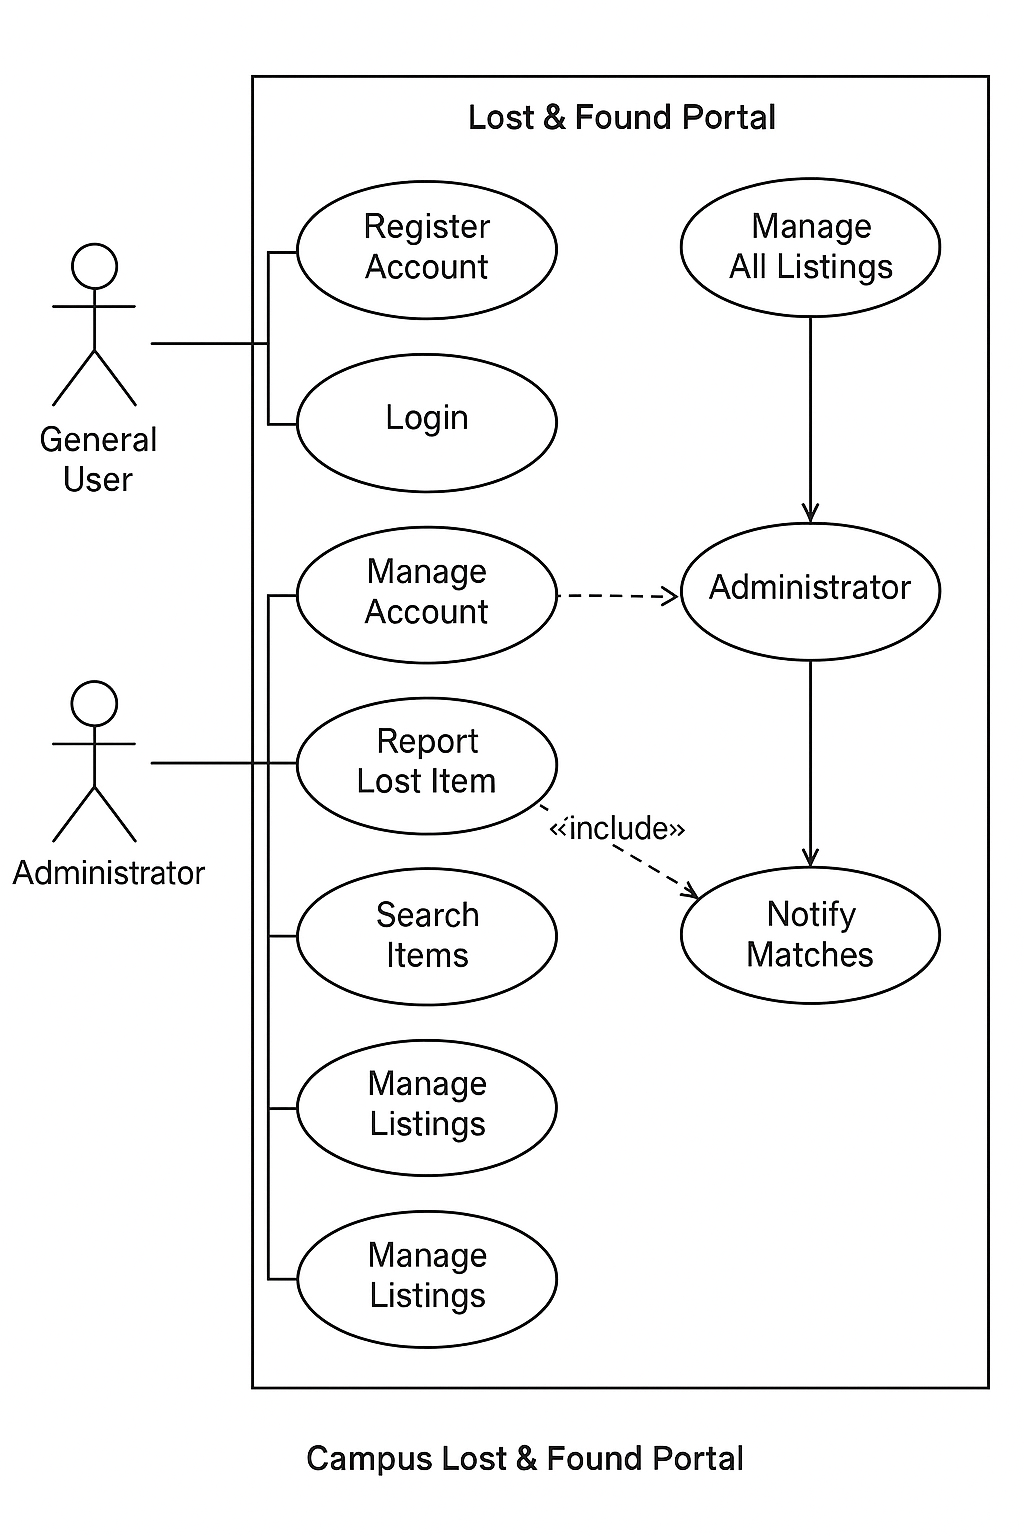
\includegraphics[width=0.8\textwidth]{use-case-diagram.png}
    \caption{Use Case Diagram for the Campus Lost \& Found Portal.}
    \label{fig:usecase}
\end{figure}
\newpage

\begin{figure}[h!]
    \centering
    % Note: Replace 'class-diagram.png' with the actual filename of your diagram.
    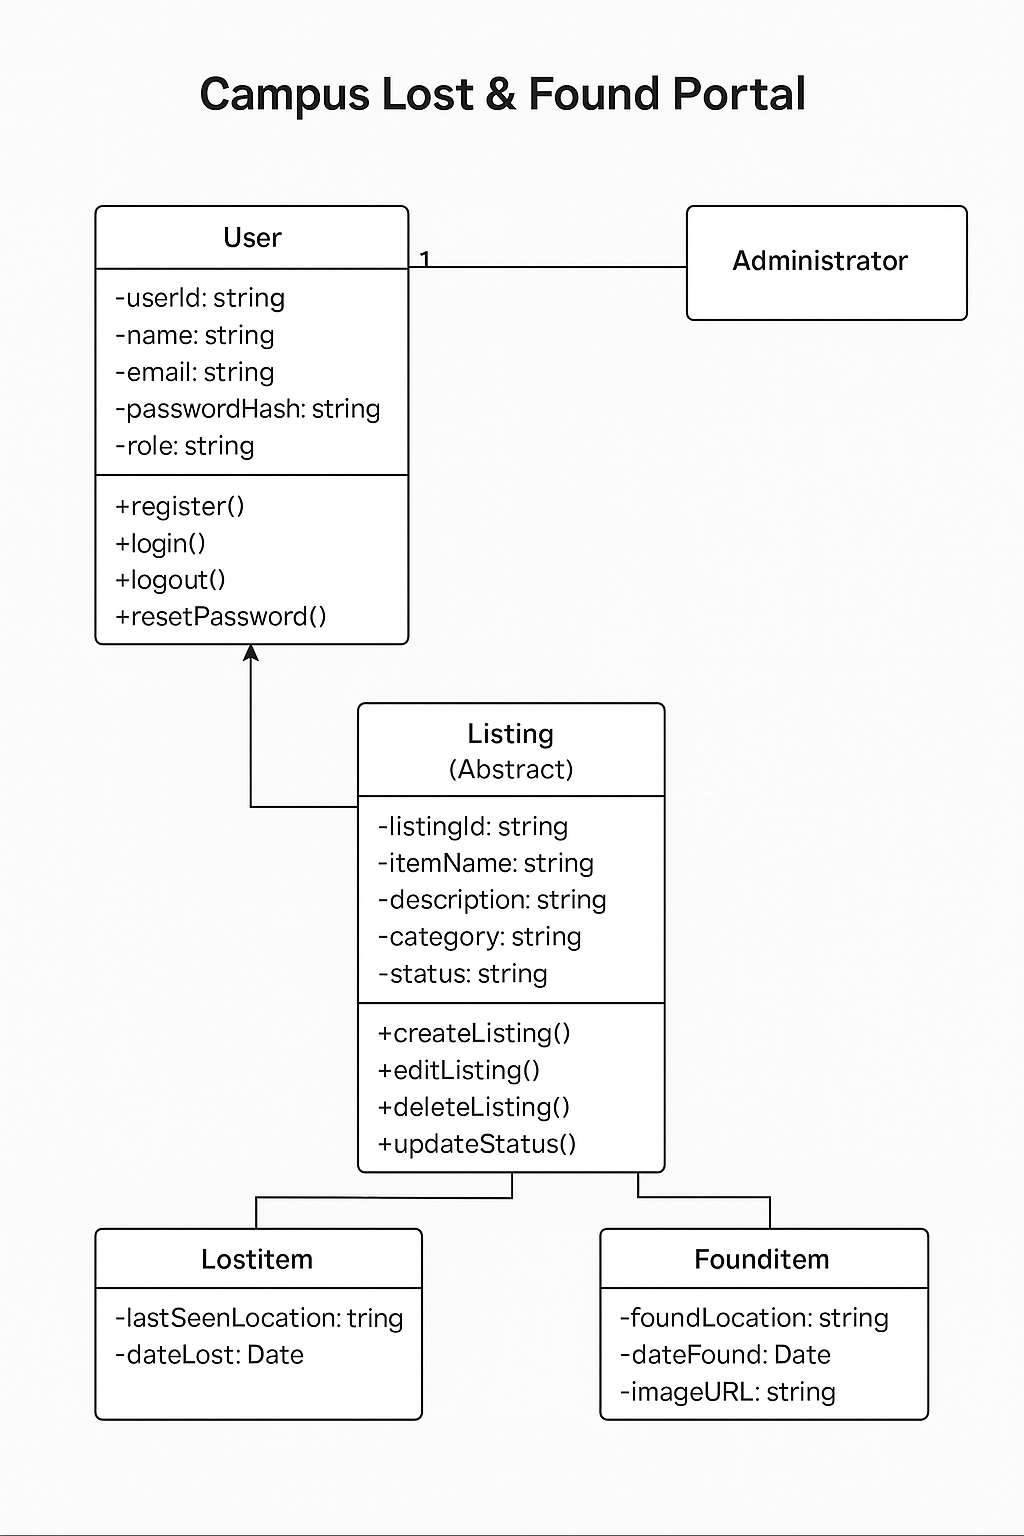
\includegraphics[width=\textwidth]{class-diagram.png}
    \caption{Class Diagram showing the main entities and their relationships.}
    \label{fig:class}
\end{figure}
\newpage

\begin{figure}[h!]
    \centering
    % Note: Replace 'sequence-login.png' with the actual filename of your diagram.
    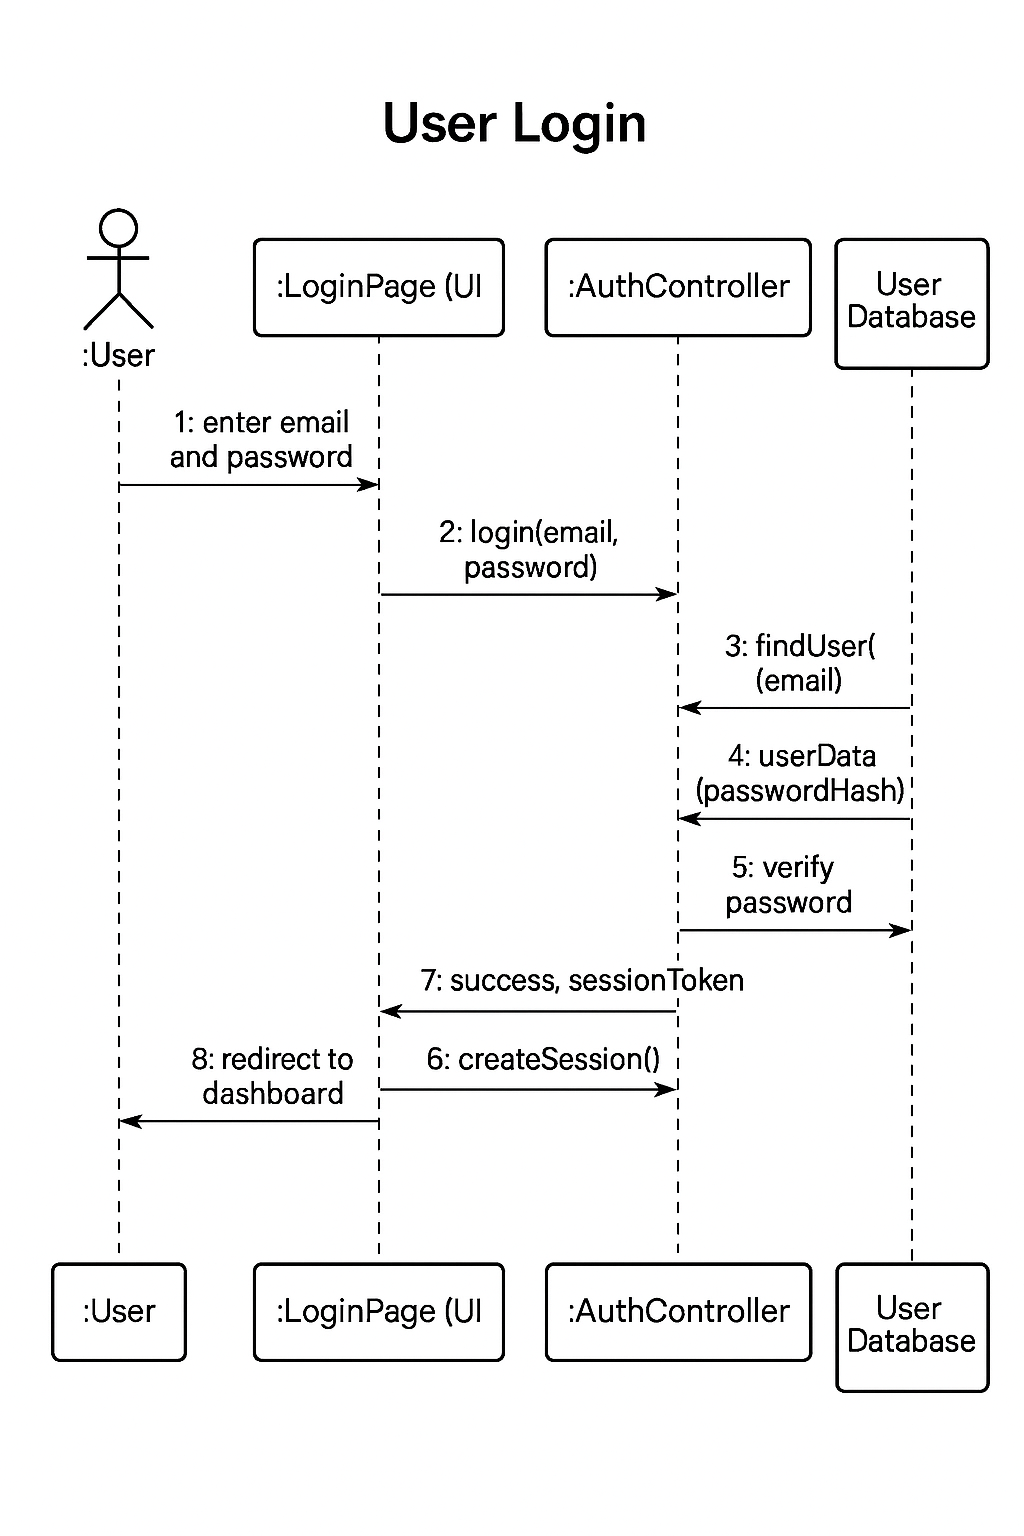
\includegraphics[width=0.9\textwidth]{sequence-login.png}
    \caption{Sequence Diagram for the User Login process.}
    \label{fig:sequencelogin}
\end{figure}

\begin{figure}[h!]
    \centering
    % Note: Replace 'sequence-report-item.png' with the actual filename of your diagram.
    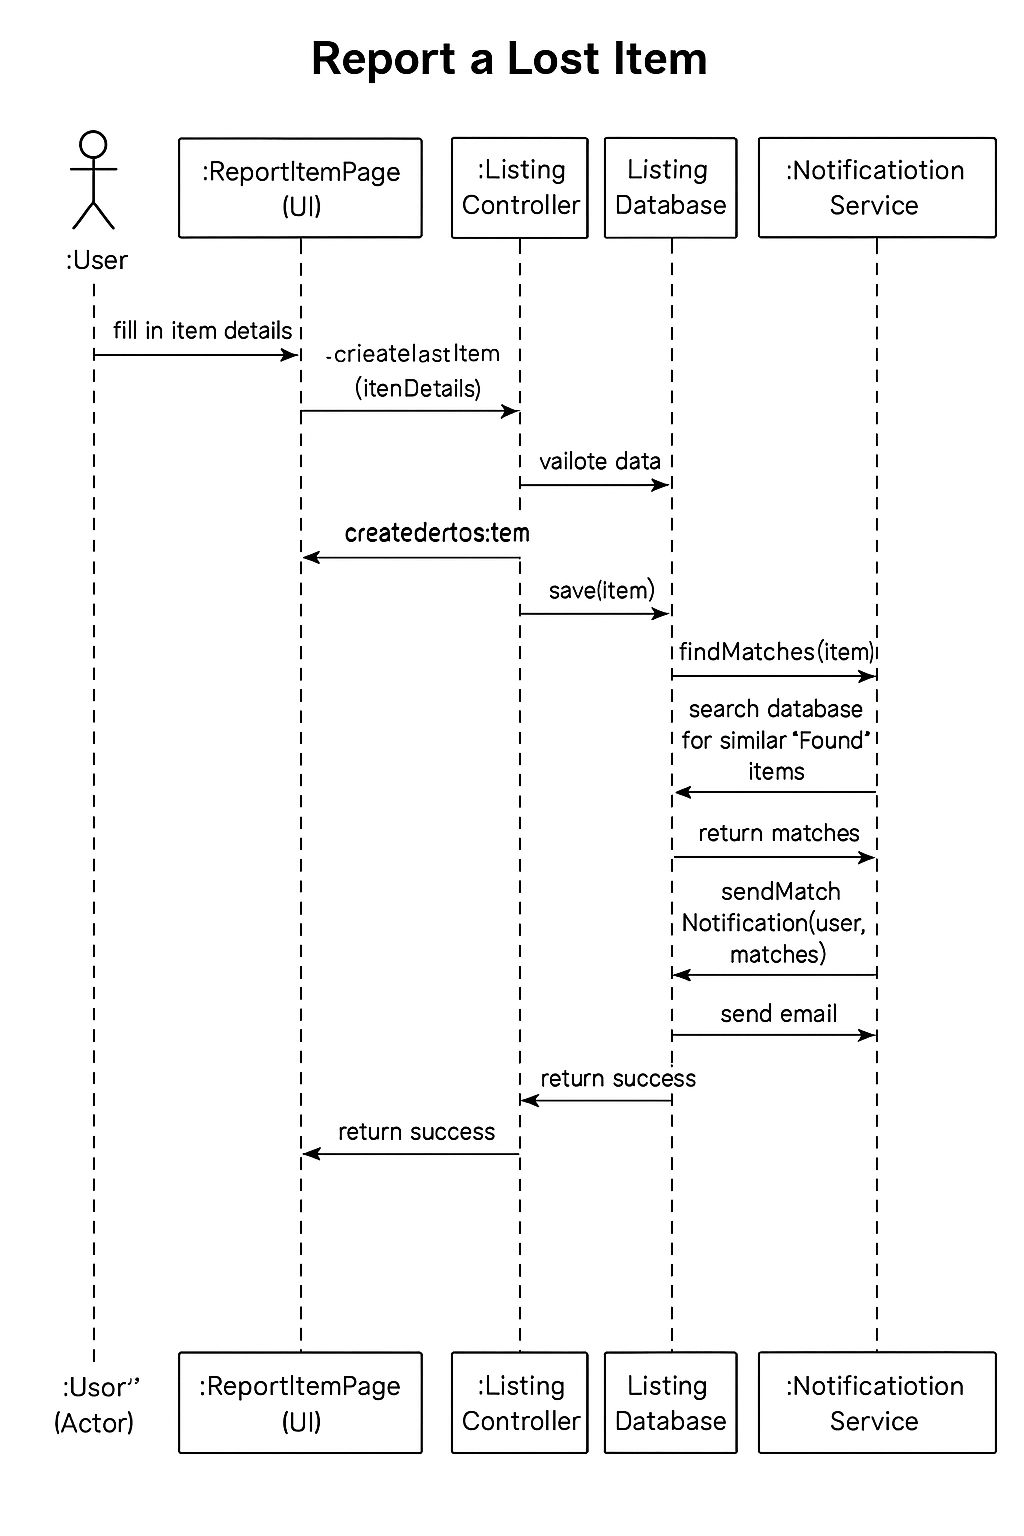
\includegraphics[width=0.9\textwidth]{sequence-report-item.png}
    \caption{Sequence Diagram for Reporting a Lost Item.}
    \label{fig:sequencereport}
\end{figure}
\newpage

\subsection{Data Flow Diagrams (DFDs)}
\begin{figure}[h!]
    \centering
    % Note: Replace 'dfd-level-0.png' with the actual filename of your diagram.
    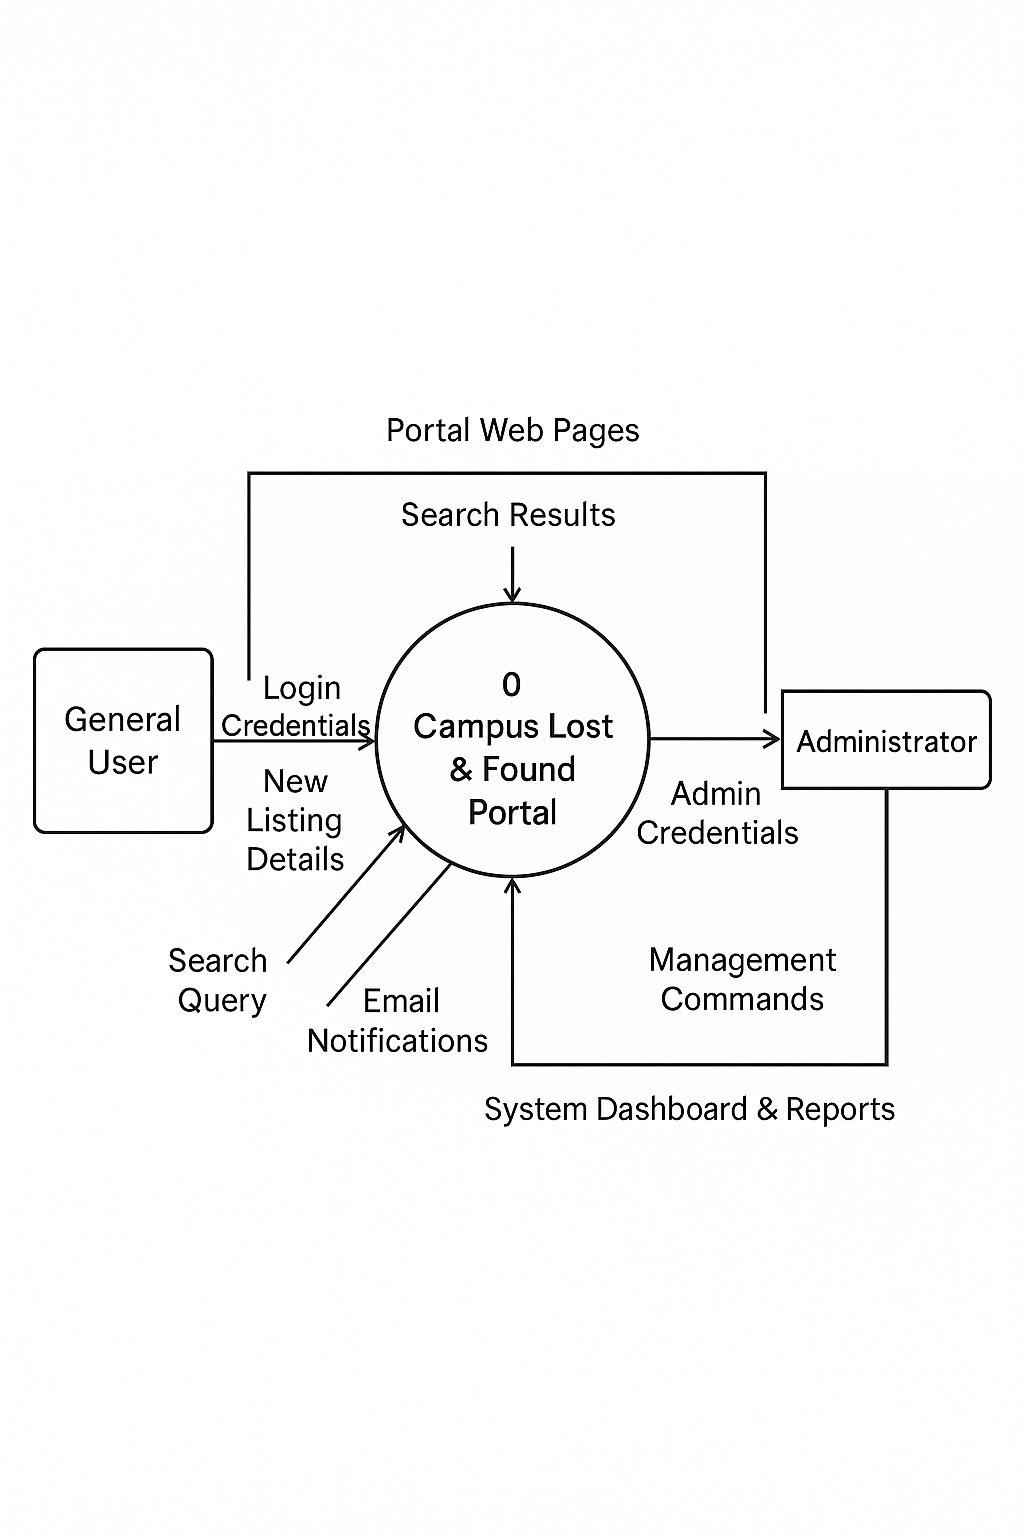
\includegraphics[width=0.8\textwidth]{dfd-level-0.png}
    \caption{DFD Level 0 (Context Diagram) for the Portal.}
    \label{fig:dfd0}
\end{figure}

\begin{figure}[h!]
    \centering
    % Note: Replace 'dfd-level-1.png' with the actual filename of your diagram.
    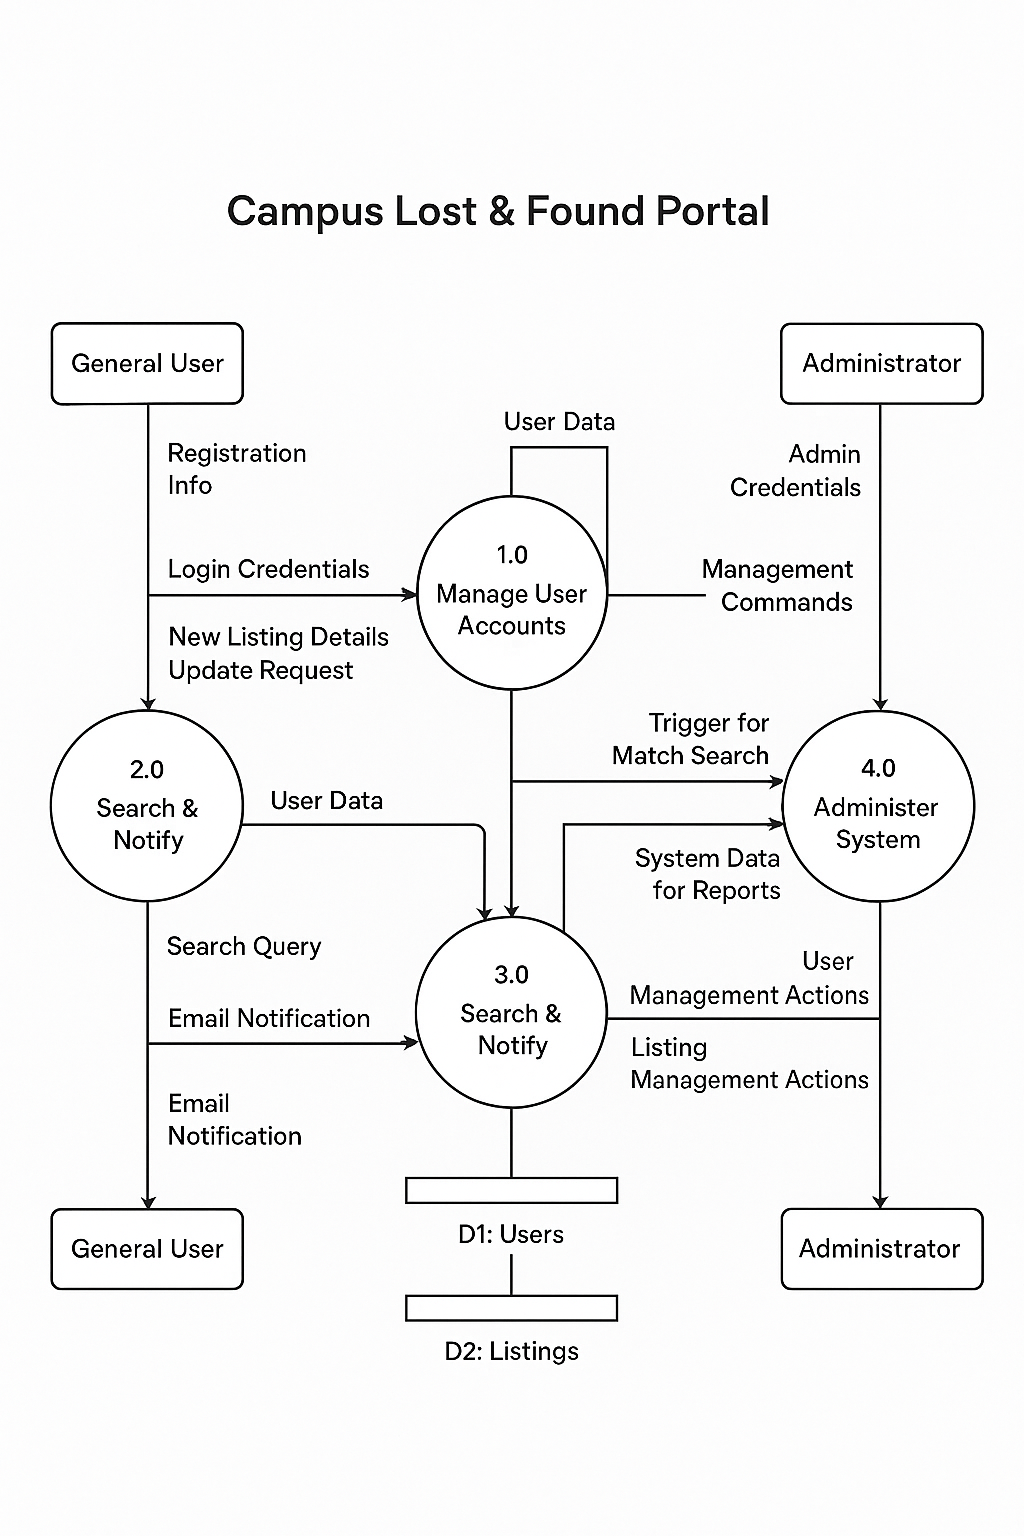
\includegraphics[width=\textwidth]{dfd-level-1.png}
    \caption{DFD Level 1 for the Portal.}
    \label{fig:dfd1}
\end{figure}
\newpage

\begin{figure}[h!]
    \centering
    % Note: Replace 'dfd-level-2.png' with the actual filename of your diagram.
    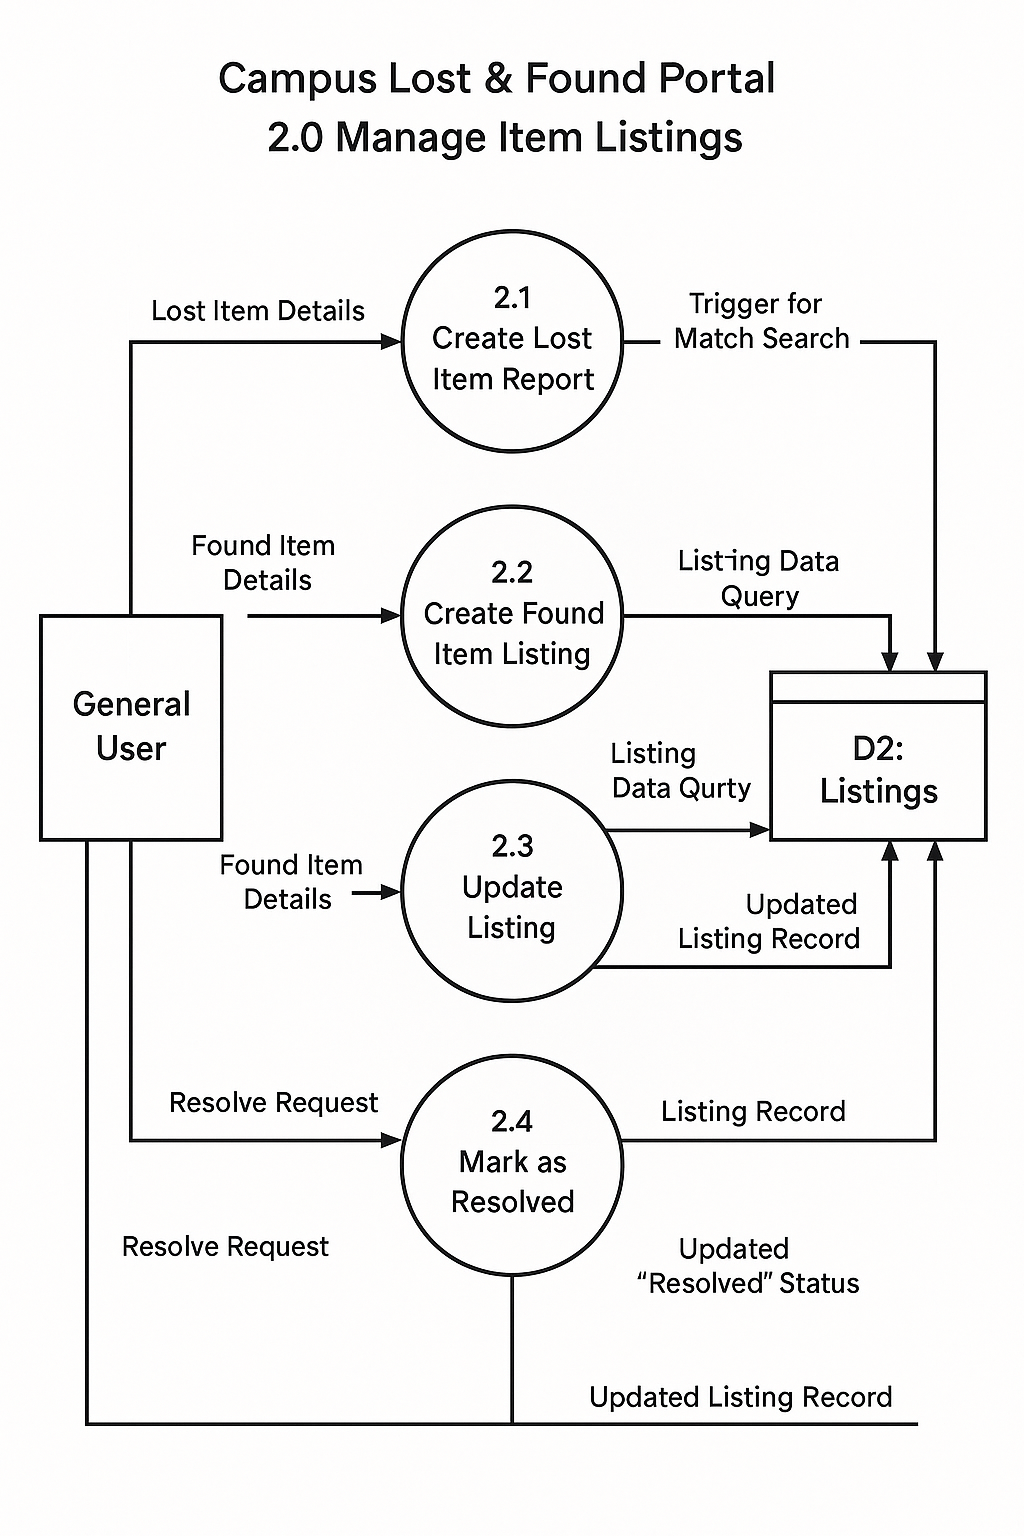
\includegraphics[width=\textwidth]{dfd-level-2.png}
    \caption{DFD Level 2 for Process 2.0 (Manage Item Listings).}
    \label{fig:dfd2}
\end{figure}


% --- Appendix C: To Be Determined List ---
\section{To Be Determined List}
\begin{enumerate}
    \item \textbf{TBD-1:} The specific process for verifying and granting Administrator privileges.
    \item \textbf{TBD-2:} The exact criteria and weighting for the automated matching algorithm (related to REQ-14, REQ-15).
\end{enumerate}

% =================================================================================
% END DOCUMENT
% =================================================================================
\end{document}
